\documentclass[12pt]{article}
\usepackage[T2A]{fontenc}
\usepackage[utf8]{inputenc}
\usepackage[english, russian]{babel}

\usepackage{color}
\usepackage{geometry}
\usepackage{indentfirst}
\textheight = 24cm
\textwidth = 16.5cm
\oddsidemargin = 0cm
\topmargin = -1.5cm
\parindent = 24pt
\parskip = 0pt

\usepackage{graphicx}
\graphicspath{{images/}}

\usepackage{amsmath, amsthm, amssymb, thmtools}

\declaretheorem[style = definition, numbered = no]{definition}
\declaretheorem[style = plain]{lemma}
\declaretheorem[style = plain]{theorem}

\usepackage{algorithmicx}
\usepackage[Algorithm, ruled]{algorithm}
\usepackage{algpseudocode}
\newcommand{\Break}{\State \textbf{break} }

\usepackage{cite}

\begin{document}
\section{Introduction}
{\color{green}
Задача построения триангуляции Делоне (ТД) $n$ сайтов-точек имеет нижнюю оценку вычислительной сложности  $O(n\log n)$.
В случаях, когда имеется некоторая дополнительная информация для множества сайтов, эта оценка может быть улучшена.
В частности, представляет интерес задача слияния двух триангуляций, когда исходное множество сайтов состоит из двух непересекающихся подмножеств $\bf{S} = \bf{S_1} \cup \bf{S_2}$, и триангуляции Делоне $Del(\bf{S_1})$ и $Del(\bf{S_2})$  исходных множеств $\bf{S_1}$ и $\bf{S_1}$ уже построены.
В \cite{Lee} описан алгоритм Ли-Шехтера слияния ТД за время $O(n)$ в случае, когда множества точек $\bf{S_1}$ и $\bf{S_2}$ линейно разделимы.
Мы рассматриваем более общую постановку задачи слияния ТД, когда множества сайтов $\bf{S_1}$ и $\bf{S_2}$ не пересекаются $\bf{S_1} \cap \bf{S_2} = \emptyset$, но перекрываются, т.е. пересекаются их выпуклые оболочки
$Conv(\bf{S_1})~\cap$ $Conv(\bf{S_2}) \ne \emptyset$.
Даны ТД $Del(\bf{S_1})$ и $Del(\bf{S_2})$, нужно построить ТД
$Del(\bf{S_1} \cup \bf{S_2})$ за время $O(n)$ в худшем случае.
}

The task of constructing Delaunay triangulation (DT) of $n$ points (which are called sites) has a lower bound of computational complexity $O(n\log n)$.
If we have some additional information for a variety of sites, this estimate can be improved.
Particularly, there are a some interest a merger of two triangulations, when the initial set of sites consists of two disjoint subsets $\bf{S} = \bf{S_1} \cup \bf{S_2} $, and the Delaunay triangulations $Del(\bf{S_1}) $ and $Del(\bf{S_2})$ are built.
There are the Lee-Schechter algorithm \cite{Lee} of TD's merger with $O(n)$ complexity in the case where the clouds of points $\bf{S_1}$ and $\bf{S_2}$ are linearly separable.
We consider a more general statement of the problem merger of TD when many sites $\bf{S_1}$ and $\bf{S_2}$ don't intersect $\bf {S_1}\cap \bf{S_2} = \emptyset$, but their convex hulls are overlaping $Conv(\bf{S_1})~\cap$ $Conv(\bf{S_2})\ne \emptyset$.
There are TDs $Del(\bf{S_1})$ and $Del(\bf{S_2})$, we should build TD $Del(\bf{S_1} \cup \bf {S_2})$ in time $O(n)$ in the worst case.

{\color{green}
В такой постановке задача слияния ТД до сих пор не рассматривалась, возможно, потому, что не представляла практического интереса.
Наш интерес к этой постановке связан с построением алгоритма для вычисления расстояния в метрическом пространстве функций двух переменных, заданных на конечных нерегулярных множествах точек.
Эта задача возникает, в частности, при анализе 3D поверхностей человеческих лиц, полученных в результате пространственного сканирования \cite{Dyshkant}.
Предложенная модель определяет расстояние между такими функциями на основе построения общей ТД.
При этом расстояние между моделями лиц определяется как минимальное по всем движениям множеств $\bf{S_1}$ и $\bf{S_2}$ на плоскости.
Таким образом, осуществляется подгонка пары поверхностей друг к другу.
И на каждой итерации подгонки выполняется слияние триангуляций.
}

In this posing, the task of TD merger has not been considered yet, perhaps because of no practical interest.
Our interest in this terms is associated with the construction of an algorithm to calculate the distance in a metric space of 	two-variable functions defined on finite sets of irregular points.
This problem goes up, for example, in the analysis of 3D human face surfaces by spatial scanning \cite{Dyshkant}.
The proposed method defines the distance between these functions based on a common TD.
The distance between the face's models is defined as the minimum of all the movements of the sets $\bf{S_1}$ and $\bf{S_2}$ on the plane.
Thus, the adjustment of two surfaces to each other is implemented.
On each iteration of adjustment there are a merger of initial triangulations.

{\color{green}
Поскольку ТД и диаграмма Вороного (ДВ) $n$ сайтов являются двойственными графами и могут быть получены один из другого за время $O(n)$, для решения задачи в принципе можно использовать известные алгоритмы Киркпатрика \cite{Kirkpatrick} и Шазеля \cite{Chazelle}.
Алгоритм Киркпатрика \cite{Kirkpatrick} строит ДВ $Vor(\bf{S_1} \cup \bf{S_2})$ перекрывающихся множеств сайтов $\bf{S_1}$ и $\bf{S_2}$ на основе слияния ДВ $Vor(\bf{S_1})$ и $Vor(\bf{S_2})$. Для решения нашей задачи нужно преобразовать исходные ТД $Del(\bf{S_1})$, $Del(\bf{S_2})$ в $Vor(\bf{S_1})$, $Vor(\bf{S_2})$, построить $Vor(S_1 \cup S_2)$ с помощью алгоритма \cite{Kirkpatrick}, а затем преобразовать $Vor(\bf{S_1} \cup \bf{S_2})$ в $Del(\bf{S_1} \cup \bf{S_2})$.
Алгоритм Шазеля \cite{Chazelle} строит пересечение двух выпуклых многогранников в 3D-пространстве.
Для его использования применительно к нашей задаче требуется построить из исходных ТД $Del(\bf{S_1})$, $Del(\bf{S_2})$ сначала ДВ $Vor(\bf{S_1})$, $Vor(\bf{S_2})$, затем выпуклые многогранники. Затем нужно построить пересечение этих многогранников с помощью алгоритма \cite{Chazelle}. После этого из многогранника получается сначала ДВ $Vor(\bf{S_1} \cup \bf{S_2})$, а после $Del(\bf{S_1} \cup \bf{S_2})$.
Таким образом, используя алгоритм \cite{Kirkpatrick, Chazelle}, мы получаем решение за 3 и 5 шагов соответственно. И хотя вычислительная сложность этих решений остается $O(n)$, их практическая реализация весьма проблематична.
В отличие от этого, предлагаемый нами алгоритм находит $Del(\bf{S_1} \cup \bf{S_2})$ непосредственно на основе слияния исходных ТД $Del(\bf{S_1})$ и $Del(\bf{S_2})$.
}

TD and Voronoi diagram (VD) are the dual graphs and they can be constructed one from other in $O(n)$.
For our problem the Kirkpatrick's algorithm \cite{Kirkpatrick} and Chazelle's algorithm \cite{Chazelle} can be used.
The first one builds VDs $Vor(\bf{S_1} \cup \bf{S_2})$ of overlapping sets $\bf{S_1}$ and $\bf{S_2}$ by merger of $Vor(\bf{S_1})$ and $Vor(\bf{S_2})$.
We should convert initial DTs $Del(\bf{S_1})$, $Del(\bf{S_2})$ conforming to $Vor(\bf{S_1})$, $Vor(\bf{S_2})$, construct combined VD $Vor(S_1 \cup S_2)$ with Kirkpatrick's algorithm and then again convert $Vor(\bf{S_1} \cup \bf{S_2})$ to $Del(\bf{S_1} \cup \bf{S_2})$.
The Chazelle's algorithm \cite{Chazelle} construct intersection of two 3D convex polyhedrons.
To solve our problem we should start with constructing from $Del(\bf{S_1})$, $Del(\bf{S_2})$ VDs $Vor(\bf{S_1})$, $Vor(\bf{S_2})$,
then convex polyhedrons.
After that we can use Chazelle's algorithm and convert combined polyhedron to combined TD $Del(\bf{S_1} \cup \bf{S_2})$ through VD $Vor(\bf{S_1} \cup \bf{S_2})$.
Thus, we obtain the solution for 3 and 5 steps using an algorithms \cite{Kirkpatrick, Chazelle} respectively.
Although the computational complexity of these decisions is $O(n)$, its practical implementation is problematic.
Contrastingly, our proposed algorithm finds $Del(\bf{S_1} \cup\bf{S_2})$ directly based on the merger of the original TD $Del(\bf{S_1})$ and $Del(\bf{S_2})$.

{\color{green}
Ещё одной причиной для прямого использования триангуляций Делоне служит то, что структура данных, описывающая ТД, обычно намного проще, чем структура ДВ.
В ТД все все ребра одного типа, и имеют конечную длину.
Напротив, в ДВ существует специальный массив, хранящий бесконечные ребра диаграммы Вороного.
Наличие этого факта существенно осложняет задачу описания алгоритмов слияния.
Это и было одной из причин для разработки алгоритма Ли-Шехтера \cite{Lee}, хотя аналогичный алгоритм для ДВ, описанный в \cite{Shamos}, был уже известен.
Таким образом, актуальна задача описания и разработки эффективного алгоритма слияния пересекающихся триангуляций Делоне.
}

Another reason for direct DT algorithms (versus VD algorithm) is that the data structures describing the DTs are usually simpler than those describing the VDs.
In the DT graphs, all the edges are of the same type --- they are segments of finite length.
In VDs, there are also rays, which are the sides of infinite Voronoi polygons.
This fact complicates the description of algorithms.
Apparently, this feature was one of the reasons for the development of the Lee-Schachter DT algorithm \cite{Lee}, although the similar VD algorithm described in \cite{Shamos} had already been known. Thus, the development and implementation of an efficient algorithm for merging overlapping DTs is still actual.

\section{Problem Definition}
{\color{green} Пусть на евклидовой плоскости задано $\bf{S}$ --- множество из
$n \ge 3$ точек, не все из которых лежат на одной прямой.
Эти точки будем называть {\it сайтами}.
}

Let $\bf{S}$ be a set of $n \ge 3$ points in the Euclidean plane which are not in the one line.
These points are called sites.

{\it Триангуляцией} конечного множества точек $\bf{S}$ называется планарный граф с вершинами из $\bf{S}$,
все внутренние области которого являются треугольниками.
Триангуляция называется {\it выпуклой}, если минимальный многоугольник, охватывающий все ее треугольники, будет выпуклым.
Далее под термином {\it грань} будем понимать только конечную треугольную грань триангуляции.
Ребро и грань называются {\it инцидентными}, если они имеют две общие вершины.
Ребра, инцидентные одной грани, называются {\it смежными}.
Ребро, имеющее менее двух инцидентных граней, называется {\it открытым}.

Окружность называется {\it пустой}, если она не содержит внутри себя сайтов.
Прямая линия, по одну сторону от которой нет сайтов, называется {\it несобственной} пустой окружностью.
Окружность, проходящая через сайт, называется {\it инцидентной} этому сайту.
{\it Ребром Делоне} называется ребро, инцидентные сайты которого имеют общую пустую инцидентную окружность.
{\it Гранью Делоне} называют грань, вершины которой имеют общую пустую инцидентную окружность.

Дадим два эквивалентных определения:

\begin{definition}
{\it Триангуляцией Делоне (ТД) $Del(\bf{S})$} множества точек $\bf{S}$ называется выпуклая триангуляция,
у которой описанная окружность каждой треугольной грани является пустой,
т.е. все грани которой являются гранями Делоне.
\end{definition}

\begin{definition}
{\it Триангуляцией Делоне} множества точек $\bf{S}$ называется выпуклая триангуляция,
у которой для каждого ребра существует пустая инцидентная сайтам-вершинам окружность,
т.е. все ребра которой являются ребрами Делоне.
\end{definition}

{\it Пучком} сайта $p \in \bf{S}$ называют множество ребер триангуляции, инцидентных сайту $p$.
Пучок сайтов будем представлять в виде двунаправленного циклического списка сайтов $p_1, \ldots, p_k$,
смежных с $p$ в триангуляции, так чтобы они шли в направлении обхода против часовой стрелки относительно $p$.

Задача слияния двух перекрывающихся триангуляций Делоне ставится следующим образом.
Даны два конечных линейно неразделимых множества сайтов $\bf{B}$ и $\bf{W}$ (считаем, что сайты раскрашены в два цвета: множество черных сайтов $\bf{B}$ и множество белых сайтов $\bf{W}$),
а также их триангуляции Делоне $Del(\bf{B})$ и $Del(\bf{W})$.
Нужно построить триангуляцию Делоне на объединенном множестве сайтов $Del(\bf{B} \cup \bf{W})$.

{\color{green}
Пример исходных данных и искомой триангуляции приведен на рис. \ref{fig:model_data}.
}

The problem of merging two overlapping DTs is presented in fig. \ref{fig:model_data}.

\begin{figure}[htb!]
	\begin{minipage}[h]{0.49\linewidth}
		\center{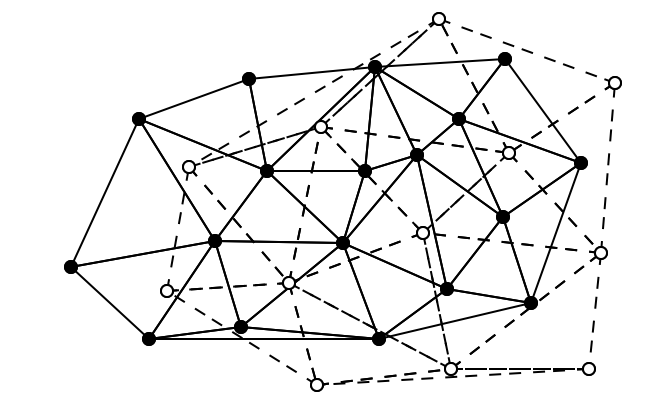
\includegraphics[width=1\linewidth]{model_data.png}}
	\end{minipage}
	\hfill
	\begin{minipage}[h]{0.49\linewidth}
		\center{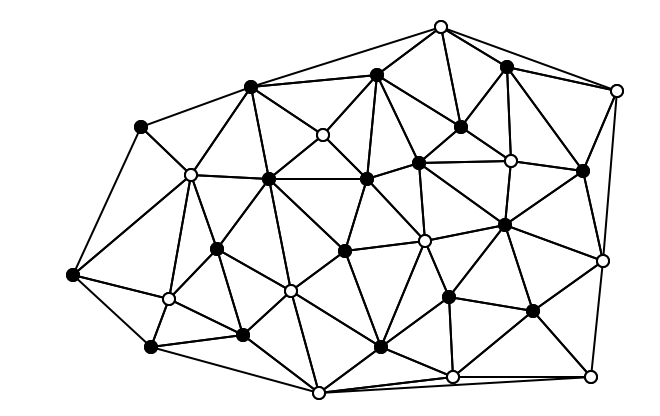
\includegraphics[width=1\linewidth]{model_res.png}}
	\end{minipage}
	\caption{Initial triangulations and combined one}
	\label{fig:model_data}
\end{figure}

\section{The Structure of the Algorithm}
{\color{green}
В объединенной триангуляции Делоне $Del(\bf{B} \cup \bf{W})$ существуют ребра двух типов:
одноцветные, которые были взяты из исходных триангуляций, и разноцветные, сайты-вершины которых взяты из разных исходных триангуляций.
}

The combined triangulation $Del(\bf{B} \cup \bf{W})$ includes one-color and two-color edges and faces depending on the colors of their incident sites. The one-color edges and faces are included in $Del(\bf{B} \cup \bf{W})$ directly from $Del(\bf{B})$ or $Del(\bf{W})$, and the two-color edges and faces are newly created.

{\color{green}
В объединенной триангуляции существуют максимальные связные одноцветные подмножества вершин и ребер,
переходящие без изменений из исходных триангуляций, которые будем называть {\it лоскутами}.
Ребра и грани, не вошедшие в лоскуты, должны быть разрушены.
Такие связные подмножества будем называть {\it разрезами}.
При построении разрезов будут удалены некоторые грани, что приведет к образованию открытых ребер.
При объединении будут образовываться новые разноцветные ребра, называемые {\it стежками}.
Максимальные связные подмножества разноцветных ребер и граней объединенной триангуляции будем называть {\it швами}.
}

Maximal one-color connected components in the combined triangulation $Del(\bf{B} \cup \bf{W})$ will be called {\it patches}.
These components are directly transferred from $Del(\bf{B})$ or $Del(\bf{W})$ without any changes.
The other one-color edges of Del(B) and Del(W), which were not included into the patches, must be destroyed during the merge, and are called {\it cuts} of the initial DTs.
During the building of cuts some faces will be destroyed and there will be some open edges.
The merge process can be considered as the extraction of patches in $Del(\bf{B})$ and $Del(\bf{W})$ and then joining the patches by two-color edges called {\it stitches}.
A maximal subset of stitches joining two patches is called a {\it seam}. 

{\color{green}
При данных определениях построение объединенной триангуляции Делоне состоит из нескольких частей: построения разрезов,
выделения лоскутов исходных триангуляций и построения швов.
}

Thus, the merge of two DTs is organized as a consecutive construction of cuts, finding of patches and creating seams.

{\it Стартером} будем называть пару разноцветных сайтов, образующих ребро Делоне,
еще не включенное в объединенную триангуляцию.
Стартер нужен для запуска процесса построения разрезов и швов.
Построение смежных стежков для стартера можно вести по разные стороны от него.
Для определенности будем полагать, что стартер имеет левый и правый сайты,
построение стежка происходит в направлении перед стартером.
На рис. \ref{pic:dir} черная жирная линия обозначает стартер, жирная пунктирная новый стежок, построенный в направлении перед стартером.

Шов может быть двух типов.
{\it Разомкнутым} швом называется шов, имеющий два стежка, принадлежащих выпуклой оболочке объединенной триангуляции,
то есть принадлежащих граничным ребрам $Del(\textbf{B} \cup \textbf{W})$.
{\it Циклическим} называется шов, имеющий только внутренние ребра объединенной триангуляции.

В процессе построения разомкнутого шва сначала находим одну его часть,
затем продолжаем движение по другую сторону стартера и находим оставшуюся часть разреза.
В циклическом шве в некоторый момент времени стартер совпадет с новым стежком,
на этом построение шва будет закончено.

Введем понятие минимального остовного дерева.
{\it Минимальным остовным деревом (МОД)} триангуляции Делоне называется ее связный подграф,
имеющий наименьшую суммарную длину ребер.
Пусть на плоскости задано $N$ точек.
{\it Евклидовым МОД (ЕМОД)} называется связный подграф,
вершинами которого являются все $N$ точек, суммарная длина всех ребер которого минимальна.
Известно, что МОД ТД является евклидовым минимальным остовным деревом для множества сайтов ТД \cite[стр. 229, 277]{Preparata}.
МОД исходных триангуляций Делоне понадобятся в процессе построения стартеров.

{\color{green}
Общая схема алгоритма слияния перекрывающихся триангуляций Делоне:

\begin{enumerate}
	\item Построить начальный стартер
	\item \label{alg_ru:seam} Построить разрез и шов от первого стартера
	\item Поиск очередного стартера
	\item Если стартер найден, перейти к пункту \ref{alg_ru:seam}, иначе закончить работу алгоритма
\end{enumerate}
}

The algorithm involves the following procedures:
\begin{enumerate}
	\item Find an initial starter
	\item \label{alg:seam} Build a cut and a seam from the starter
	\item Try to find the next starter
	\item If the next starter is found, then go to step \ref{alg:seam}; otherwise, stop
\end{enumerate}

\newpage
\bibliographystyle{utf8gost705u}
\bibliography{tri_article}{}

\end{document}